%*************************************************************************************************************
%*************************************************************************************************************
%**************************Journal of Systems Science and Complexity (JSSC)***********************************
%*************************************************************************************************************
%*************************************************************************************************************
% This is the model of the standard format of articles published on Journal of Systems Science and Complexity.
% Please read through the whole guidance marked by "%" before you type according to the guidance.
% After "\end{document}", an article is attached just for an example and you can refer to it.
%*************************************************************************************************************

\documentclass{jssc}

%************************************************************
%Beginning of the head of the tex file of JSSC. You can skip.
%************************************************************

%----------------------------------------------------------------------

\def\textsubscript#1%
{$_{\text{#1}}$}
\newcommand*\supercite[1]{\textsuperscript{\cite{#1}}}
%The definition of superscript about the cited references
\def\cdd{\mbox{\boldmath$\cdot$}~}
% name defs.tex
%\catcode`@=11
\def\vsp{\vspace{1mm}}
\def\no{\nonumber}
\def\q{\quad} \def\qq{\qquad}
\def\ee{{\rm e}}
\newcommand{\rulex}{\hfill\rule{1mm}{3mm}}
\def\ay{\arraycolsep=1.5pt}
\def\d{\displaystyle}
\def\dfrac{\displaystyle\frac}
\input{amssym.def}
\include{graphix}

%---------------------------------------------------------------------
%************************************************************
%End of the head of the tex file of JSSC.
%************************************************************


%%-------------------   Beginning of  Author's Definitions  -------------------%%
%%                     Note: You may add your own definitions here.

%************************************************************




%************************************************************
%Some user-defined commands, you can add more
%************************************************************



%************************************************************

%%-------------------     the end of  Author's Definitions    -------------------%%



%*************************************************************************************************************
%*************************************************************************************************************
%*************************************************************************************************************
%***Beginning of the article! Please fill the content of your articles according to the guidance.
%*************************************************************************************************************
%*************************************************************************************************************
%*************************************************************************************************************
\setcounter{page}{1}
\input jsscN.tex
\begin{document}

%*************************************************************************************************************
% \biaoti{THE CAPITALIZED TITLE OF YOUR ARTICLE$^*$}{The list of authors' names with the LAST NAME capitalized
% and the authors' names should be separated by "\cdd"}{the first author's name \\ the first author's affiliation
% and Email address\\ the second author's name\\ the second author's affiliation. More can be listed like this.}
% {$^*$ The titles and numbers of the foundations that support this article.}
%*************************************************************************************************************
\title{A Template for Journal$^*$}%%%   Main Title of your paper  %%%
{\uppercase{Surname1} Firstname1 \cdd \uppercase{Surname2}
Firstname2 \cdd \uppercase{Surname3} Firstname3}%%% The names of the authors  %%%
{\uppercase{Surname1} Firstname1 ({\bf Identify the corresponding author of this article.})\\
Address 1; Address 2.  Email: XXXXX. \\   % Academy of Mathematics and Systems Science, Chinese Academy of Sciences, Beijing $100190$, China
\uppercase{Surname2} Firstname2   \cdd \uppercase{Surname3} Firstname3 \\
Address 3; Address 4.  Email: XXXXX; XXXXX.}%\\ %%% The address of the authors  %%%
{$^*$This research was supported by \ldots under Grant No./Nos.
\ldots.\\
{$^\diamond${\it This paper was recommended for publication by Editor . }}
 }

%*************************************************************************************************************
%The submission date of your article. For example: \drd{Received: June 8, 2006}
%*************************************************************************************************************
\drd{DOI: }{Received: x x 20xx}{ / Revised: x x 20xx}

%*************************************************************************************************************
% The page header of the article.
% \dshm{Year}{Volume}{The capitalized RUNNING HEAD of your article with less than 48 letters}{The capitalized
% AUTHORS list with $\cdot$ separating different names or one can type "The name of the first author et al."
% if there are more than 4 authors.}
%*************************************************************************************************************

\dshm{20XX}{XX}{ }{A TEMPLATE FOR JOURNAL}{\uppercase{Surname1
Firstname1} $\cdd$ \uppercase{Surname2 Firstname2} $\cdd$
\uppercase{Surname3 Firstname3}}

%*************************************************************************************************************
% \dab{The abstract}{Keywords}
%*************************************************************************************************************
%-------------------------------------------------------------------------
\Abstract{Please make sure NO reference number in your
Abstract since it is misunderstood independent of full text.}      % the abstract

\Keywords{Aaaa, bbbb, cccc. (Please note the keywords by the way a-z.)}        % the keywords

%\MRSubClass{05B05, 05B25, 20B25}      % MR(2000) Subject Classification

%\baselineskip 15pt

\section{Introduction}

\subsection{A Subsection}

Please make sure that your paper contains correct reference sequence
(If NOT, please resort them according to its appearance sequence,
not alphabetical order. Moreover, please make sure that each
bibliographical item is labelled and that these items are recalled
using the command \verb|\cite{\cdots}|, such as \cite{ref1,ref2},
and \cite{ref3,ref4,ref5}).

All equations, theorems, definitions, lemmas, propositions,
assumptions, corollaries, examples, remarks, etc. would be better to
be numbered consecutively and unrepeatedly within each section. For
example, Definition 2.1, Lemma 2.2, Theorem 2.3 $\cdots$.

Notice the Greek capital letter required for your article must be
italic. For example, ${\it \Gamma}, {\it \Theta}, {\it \Lambda},
{\it \Psi}, {\it \Omega}, \cdots$. Please make sure that the
classified text in your paper are cited by the labels{}\,$1) $,
$2) $, $3)$, $\cdots$, (i), (ii), (iii),$\cdots$, or (h), (i),
(g),$\cdots$. In addition, please make sure that the elements in a
sequence list two items before an ellipsis is added,
 such as $\{f(x_i),\ i=1,2,\cdots,n\}$,\ $y_1<y_2<\cdots<y_n$, $A=A_1+A_2+\cdots+A_m$,\  $\cdots$.


References cited together in the text should be arranged
chronologically, e.g. the results on target aggregation of
first-order agent model\supercite{ref3}$\cdots$

Use \verb|\label| and \verb|\ref| or \verb|\eqref| to automatically
cross-reference sections, equations, theorems and theorem-like
environments, tables, figures, etc.

In all text and formulas, Notice the Greek capital letter must be
italic.

\begin{theorem}[see \cite{ref2}] \label{th:1.1} %Theorem 1.1 could be recalled by using Theorem \ref{th:1.1}
The statements of theorems, lemmas, propositions, corollaries, etc.
are set in italics, by using
\begin{verbatim}
\begin{theorem/lemma/proposition/corollary/remark/example}
\end{theorem/lemma/proposition/corollary/remark/example}.
\end{verbatim}
\end{theorem}

\proof Observe that \ay
\begin{eqnarray}\label{E:1.1}
AAAAAAAAAA = BBBBBBBBBBB.
\end{eqnarray}
Now apply induction on $n$ to \eqref{E:1.1}$\cdots$   \rulex


\begin{remark}\label{re:1.2}
Remarks, Assumption, Definition, Conjecture, Examples, Problems,
Algorithm, etc. are set in roman type.
\end{remark}

\section{Some Patterns}

\subsection{Figure}

%Please make sure that the mathematical symbol is consistent in the figures and your paper.
%\centerline{\includegraphics[scale=1.2]{actmark.eps}}
%\centerline{\small Figure 1\quad Journal mark}

\begin{center}
  \centerline
  {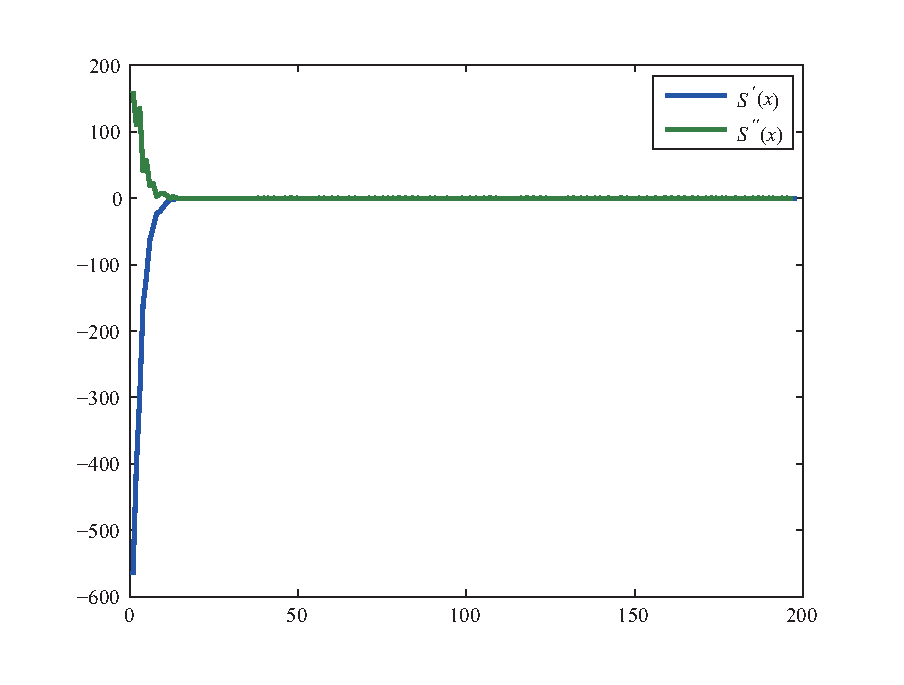
\includegraphics[scale=0.5]{1.eps}}
\centering{\small {\bf Figure 1}\ \ Aaa bbb ccc \label{fig1}}
\end{center}


\begin{center}
\centering \subfigure[The estimated function $g(\cdot)$]{
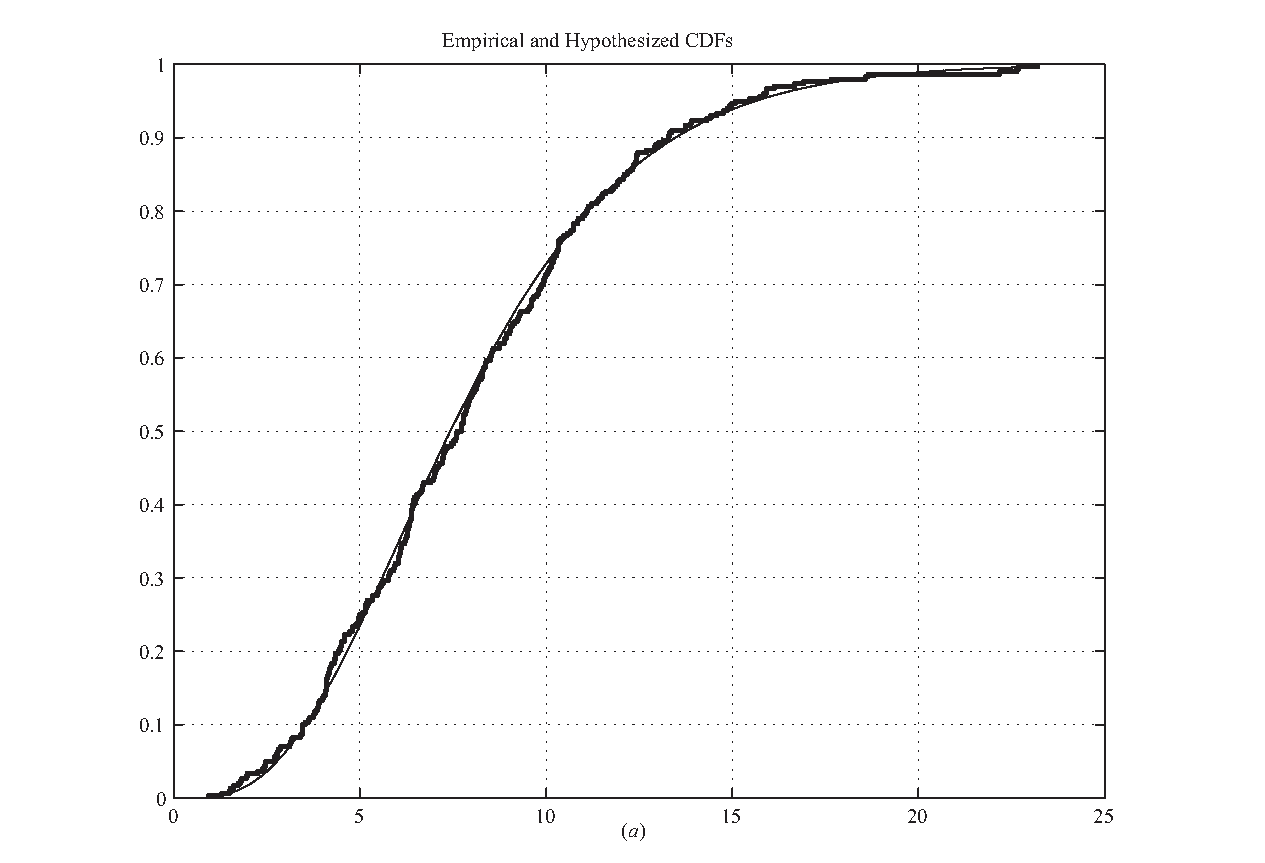
\includegraphics[scale=0.3]{2.eps}
\label{fig:subfig1} } \subfigure[The scatter plot of residuals]{
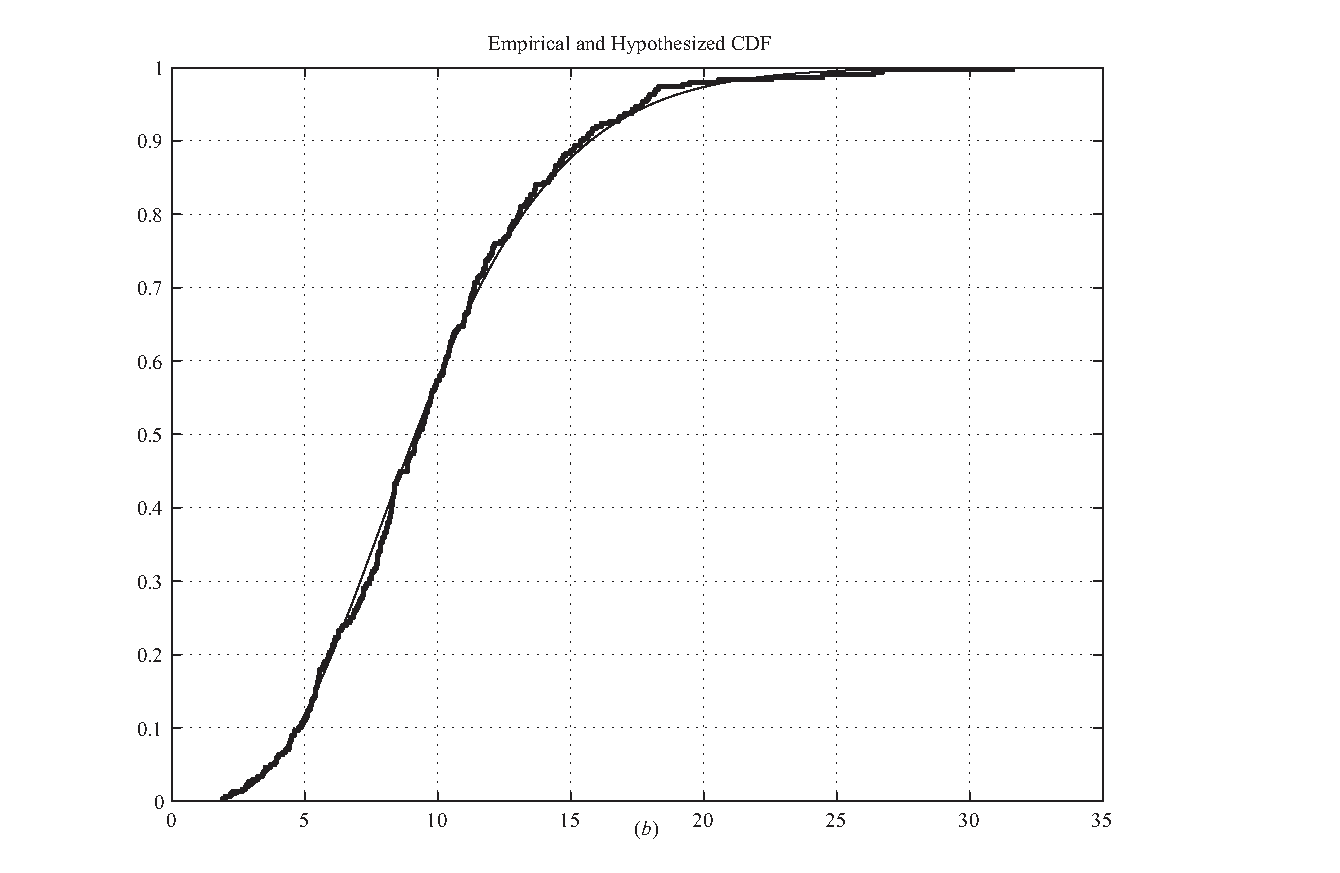
\includegraphics[scale=0.3]{3.eps}
\label{fig:subfig2} } \centerline {\small \parbox[t]{1.7cm}{\bf
Figure 2}
\parbox[t]{10.5cm}
 {The estimated function $\widehat{g}(\cdot)$ (Figure(a))
 and the corresponding scatter plot (Figure(b)) of the residuals,
  where $Y = medv-mean(medv)$, $Z$ = (\textit{rm}, $\log$(\textit{tax}), \textit{ptratio},
  $\log$(\textit{lstat}))$^\tau$}\label{fig2}}
\end{center}

\newpage
\subsection{Table}

\begin{center}\setlength{\tabcolsep}{5pt}  %���ڱ��о�
\renewcommand{\arraystretch}{1.0}%���ڱ��о�
{\small
    \begin{center}
    \centerline{\small {\bf Table 1}~~Aaa bbbbb ccc}\vskip 1mm
    \label{Tab:MSE}

    {\small
    \begin{tabular*}{6.5cm}{cccccccc}
        \hline
        &\multirow{2}{*}{$\rho$}   &\multicolumn{2}{c}{AR(1)} &   \multicolumn{2}{c}{MA(1)} &    \\

\cmidrule(r){3-4}\cmidrule(r){5-6}
                 &           & $\theta_{0}$ & $\beta_{0}$ & $\theta_{0}$ & $\beta_{0}$   \\
        \hline
            &0.6   &0.0037    &2.1503    &0.0071    &2.1247   \\
            &0.1   &0.0034    &1.8573    &0.0034    &1.7147   \\
            & 0.0   &0.0031    &1.8490    &0.0030    &1.6400   \\
            & 0.1   &0.0033    &2.0329    &0.0035    &2.1271   \\
      \hline
    \end{tabular*}}
\end{center}}
\end{center}



\subsection{Formula Format}

\ay
\begin{eqnarray}\label{E:1.2}
AAAAAAAAAA &=& BBBBBBBBBBB\nonumber \\
           && + CCCCCCCCCC\nonumber \\
           &=& DDDDDDDDDDDDD.
\end{eqnarray}
%%The formula you have entered is too long, perform one or more line feed operations.
\ay
\begin{eqnarray}\label{E:1.3}
&&AAAAAA =(A+B)-\big(B^{-2^A}+1\big)D-C,\nonumber \\
&&BBBBBBBBB=AA-BB+\bigg\{\frac{A}{B}+
\dfrac{B^2-C+\frac{A}{D}}{CC+AD}\bigg\}-CCCC\nonumber \\
&&\hspace{3cm}+DDDDD,\nonumber \\
&&DDDDDDDD={\it \Omega}A+{\it \Phi}_{2}.
\end{eqnarray}
%%Left justifies the multiple lines of formula.
%% Determine and set the size of the brackets using this formula, e.g.(),\big, \bigg.
\begin{eqnarray}\label{E:1.4}
A_{1}=B^{\rm T},\q A_{2}=C, \q A_{3}=D.
\end{eqnarray}
%% the formulas which are placed side by side are separated by \quad;
Notice that the transpose of a matrix must be used by $^{\rm T}$,
the type of the exponent value is ${\rm e}$.
\begin{displaymath}
 AA=\left\{
                   \begin{array}{ll}
                     BBB, \ & C=DD, \\
\\
                     0,\  & \mbox{otherwise}.
                   \end{array}
                 \right.
 \end{displaymath}
%% Indicates how items are aligned within the formula.


\begin{equation}
\begin{array}[b]{ll}
\|\tilde{u}^{y}(\cdot,t)\|_{L^{1}}&\leq
\ee^{\bar{\beta}t}\|u_{0}\|_{L^{1}}
+\d\int_{0}^{t}\ee^{\bar{\beta}(t-s)}\bigg\|\dfrac{f(\cdot,s)}{y(s)}\bigg\|_{L^{1}}ds \\
&\leq \ee^{\bar{\beta}t}\|u_{0}\|_{L^{1}}+\d\int_{0}^{t}\ee^{\bar{\beta}(t-s)}\dfrac{\|f(\cdot,s)\|_{L^{1}}}{y(s)}ds \\
&\leq
\ee^{\bar{\beta}T}\bigg(\|u_{0}\|_{L^{1}}+\dfrac{\|f\|_{L^{1}(Q)}}{\delta}\bigg)\doteq
r_{0}.
\end{array}
\end{equation}
%%Please make sure that you put the command '\displaystyle' in front of the formula sign \sum,\int \frac in Array environment.

\section{Conclusions}

The last section is Conclusions.

\section*{Conflict of Interest}

The authors declare no conflict of interest.

%\noindent Please confirm the following statement:

%1) If you are an editorial board member/managing
%editors/editor-in-chief for Journal of Systems Science $&$
%Complexity, please fill in the following information in this
%section: ``XX is a youth/an editorial board member/managing
%editors/editor-in-chief for Journal of Systems Science $\&$
%Complexity and was not involved in the editorial review or the
%decision to publish this article. All authors declare that there are
%no competing interests."

%2) If you are not an editorial board member/managing
%editors/editor-in-chief for Journal of Systems Science and
%Complexity, please fill in the following information in this
%section: ``The authors declare no conflict of interest. ''







\section*{Acknowledgements}
{\rm Thanks $\cdots$}

Please thank the name of anonymous people who make contributions to
this article. If you don't want it, please delete it.



\begin{thebibliography}{199}

\bibitem{ref1} %% Journals %%  surname(s), initial(s),  article, journal, year, volume, relevant page numbers.
Lorenzini D and Tucker T J, The equations and the method of
Chabauty--Coleman, {\it Invent. Math.}, 2002, {\bf 148}: 1--46.

\bibitem{ref2}
Jadbabaie A, Lin J, and  Morse A, Coordination of groups of mobile
agents using nearest neighbor rules, {\it IEEE Trans. Automatic
Control}, 2003, {\bf 48}(6): 988--1001.

\bibitem{ref3} %% Books %% surname(s), initial(s), title, publisher, place of publication, year.
Godsil C, Royle G, Morse A, et al., {\it Algebraic Graph Theory},
Springer-Verlag, New York, 2001.

\bibitem{ref4} %%Conference Proceedings%% surname(s), initial(s),  title, conference name, place of conference, year.
Michal F and Tami T, Approximate strong equilibrium in Job
Scheduling Games, {\it Proceedings of the $1$st International
Symposium on Algorithmic Game Theory}, Eds. by  Monien B and
Schroeder U P, Paderborn, 2008.

\bibitem{ref5} %%Dissertation%% surname(s), initial(s), title, place of publication, place, year.
Che Y W, $H_\infty$ analysis method for the small signal stability
of power system, Master's degree thesis, Tsinghua University,
Beijing, 2007.

\bibitem{ref6}
Test

\bibitem{ref7}
Test

\end{thebibliography}
%%Please make sure that your given name is abbreviated as the first capital letter, such as Zhang X T, Tami T,...

\section*{Appendix}

\setcounter{equation}{0}
\renewcommand\theequation{A.\arabic{equation}}





\end{document}

The following is an example you can refer to.


\title{An Improved Sensor Fault Diagnosis Scheme Based on TA-LSSVM and ECOC-SVM$^*$}%%%   Main Title of your paper  %%%
{\uppercase{Gu} Xiaodan \cdd \uppercase{Deng} Fang \cdd \uppercase{Gao} Xin \cdd \uppercase{Zhou} Rui}%%% The names of the authors  %%%
{\uppercase{Gu} Xiaodan\\
 \emph{School of Automation, Beijing Institute of Technology, Beijing $100081$, China;
Department of Information Equipment, Equipment Institute of PLA,
Beijing $101416$, China.} Email: x$\_$dan$\_$2002@163.com.\\
 \uppercase{Deng} Fang (Corresponding author) \cdd \uppercase{Gao} Xin \cdd \uppercase{Zhou} Rui\\
 \emph{School of Automation, Beijing Institute of Technology, Beijing $100081$, China.}\\
  Email:   dengfang@bit.edu.cn; xin.gao1991@qq.com; 2120130999@bit.edu.cn.} %%% The address of the authors %%%
{$^*$This research was supported in part by the National Natural
Science Foundation of China
 under Grant Nos. 61304254, 61321002 and 61120106010,
  and in part by the Key Exploration Project under Grant No. 7131253.\\
{$^\diamond${\it This paper was recommended for publication by
Editor SUN Jian. }}}

%*************************************************************************************************************
%The submission date of your article. For example: \drd{Received: June 8, 2006}
%*************************************************************************************************************
\drd{DOI: 10.1007/s11424-017-6232-3}{Received: 12 October 2016}{ /
Revised: 24 November 2016}

%*************************************************************************************************************
% The page header of the article.
% \dshm{Year}{Volume}{The capitalized RUNNING HEAD of your article with less than 48 letters}{The capitalized
% AUTHORS list with $\cdot$ separating different names or one can type "The name of the first author et al."
% if there are more than 4 authors.}
%*************************************************************************************************************

\dshm{2018}{31}{A TA-LSSVM AND ECOC-SVM BASED FAULT DIAGNOSIS
SCHEME}{\uppercase{Gu Xiaodan}, et al.}

%*************************************************************************************************************
% \dab{The abstract}{Keywords}
%*************************************************************************************************************
%-------------------------------------------------------------------------
\Abstract{Monitoring the operational state of sensors promptly
 and the  accurate diagnosis of faults are essential. This paper proposes
  an improved fault diagnosis scheme for sensors, which includes both fault
   detection and fault identification. Firstly, trend analysis combined with
    least squares support vector machine (TA-LSSVM) method is proposed and
    implemented to detect faults. Secondly, an improved error correcting
    output coding-support vector machine (ECOC-SVM) based fault identification
     method is proposed to distinguish different sensor failure modes.
     To demonstrate the effectiveness of the proposed scheme, experiments
     are conducted with an MTi-series sensor, and some comparisons are made
      with other fault identification methods. The experimental results
      demonstrate that the proposed fault diagnosis scheme offers an essential
      improvement with detection real-time property and better identification accuracy.}  % the abstract

\Keywords{ECOC, fault detection, fault identification, SVM, TA.}        % the keywords

%\MRSubClass{05B05, 05B25, 20B25}      % MR(2000) Subject Classification

%\baselineskip 15pt
\section{Introduction}


Sensor are primary instruments for receiving a wide range of
information, and serve  as fundamental components in systems over an
extensive variety of fields. Sensors play a particularly essential
role in automatic control systems because the accuracy of output
measurements would affect the operation of the entire system, and
sensor faults may result in incorrect decisions if not promptly
detected. In this way, the safety and productivity of a system are
threatened. Therefore, the operational states of sensors must be
monitored, and faults diagnosed in a timely manner. In addition,
sensor monitoring and fault diagnosis is of substantial benefit for
system maintenance.

Although some model-based fault diagnosis theory have been well
established,  e.g., parity space approach, diagnostic observer,
fault detection filter\supercite{Ding2013Model,Yin2016State}, at
many times it is still difficult to establish mathematical model by
means of the first principles. On the other hand, a large amount of
data from sensor measurements are often available. Motivated by this
observation, it is of great interest to design fault diagnosis
schemes only based on the available data\supercite{Yin2016Fault}.

Numerous data processing methods have been employed for detecting
sensor faults directly by analyzing the data provided by the
sensor\supercite{1Wang2009data,YinDescriptor}. Generally, these
methods function in the following manner. The faults to be
identified are first listed. Then, correlations between the data
provided and the faults to be identified are established. This
correlation can be achieved using mechanical models, black box
models such as neural networks and hidden Markov models, and
statistical techniques such as discriminant analysis and support
vector machine (SVM). However, complex correlations will restrict
the applicability of many models and techniques. In this context,
trend analysis can be a good choice. Trends can reflect the
development rate and direction of the important parameters in the
system, which can be an effective method for the early diagnosis of
faults. Most methods employed to extract trends involve
approximating the signal, and thus data compression and regression
algorithms are needed. In a recently proposed
scheme\supercite{2Maurya2010aframework}, an interval-halving
algorithm was employed to capture the smoothness using the method of
unimodal smooth segments to approach the signal, and achieve greater
data compression. However, this algorithm performs slowly when
extracting sensor fault trends. Therefore, the trend fitting
algorithm requires further optimization. On the other hand, because
least squares SVM (LSSVM) is solved by linear equations, its
computation is very efficient. In addition, the method provides
satisfying results when employed for regression, which is
demonstrated by its wide application, e.g., time-to-failure
forecasting, reliability of operating components, and nonlinear
process
modeling\supercite{3Marcio2008,4Vong2011engine,5li2010research}.
Therefore, in the present study, trend analysis employing LSSVM
regression (TA-LSSVM) is used for fault detection.

When a sensor fault occurs, fault compensation should be conducted
according to the type of the fault. Therefore, the fault recognition
process is essential. Broadly speaking, fault identification
involves a pattern recognition process consisting mainly of two
parts, i.e., feature extraction and mode classification. Commonly
employed feature extraction techniques include two types: Linear
algorithms such as principal component analysis
(PCA)\supercite{6Jolliffe1986principal,7Chuang2015colorimetric} and
linear discriminant
analysis\supercite{8Acquah2016identifying,9JIN2010DISCRIMINANT}, and
nonlinear algorithms such as kernel
PCA\supercite{10scholkopf1998nonlinear}, generalized discriminant
analysis\supercite{11Liang2014PARAMETRIC,12baudat1990generalized},
and nonlinear wavelet
transformation\supercite{13Mercorelli2007DENOISING,14feng2008sensors}.
For mode classification, classification process commonly involve
multiple classification, while machine learning algorithms are often
designed for binary classification. A commonly employed solution to
this problem is to divide a multiple classification process into a
number of binary classification processes, and error correcting
output codes (ECOC) can be used to do this. ECOC is a useful coding
approach for correcting error data in transmission. Dietterich and
Bakiri in 1995 first proposed to use this algorithm to extend binary
classifiers for multi-class classification process. This method
proved to be simple and highly accurate, and has been widely applied
in various fields\supercite{guosuDeng2015Sensor}. When combined with
classifiers, through the coding matrix, it can output the
corresponding class of the input data combined with classifiers. In
addition, It is noted that the sensor fault identification problem
is truly a classification issue involving small samples, and the SVM
algorithm has demonstrated a significant generalization ability as
well as the ability to accommodate nonlinear
data\supercite{17Cortes1995Support}. Therefore, in the present study
SVM is applied in combination with ECOC to conduct the sensor fault
identification process.

In this paper, TA-LSSVM is employed for sensor fault detection, and
an
 improved ECOC-SVM based sensor fault identification method is proposed
 to distinguish different failure modes. The methods used in this paper
 are introduced in Section 2. In Section 3,
 the proposed scheme is applied in an MTi-series sensor, and the experimental
  results are presented. Finally, Section{}\,4 concludes the paper.


%%%%%%%%%%%%%%%%%%%%%%%%%%%%%%%%%%%%%%%%%%
\section{Methods and Schemes}

\subsection{Sensor Fault Detection Using TA-LSSVM}

\subsubsection{Preliminaries for Fault Detection}

 TA aims to describe sensor signals as a series of identifiers based
  on primitives that are characterized according to the first and second derivatives
   of the trend, which offers a concise means of expression for the typically large
   amounts of data involved. Data collected from sensors is sequentially subjected to
    the following steps: Qualitative modeling, trend extraction of key variables,
    and trend identification. In this way, time series are transferred into primitives
     sequence, as shown in the following formula (\ref{formula1}).
\begin{equation}\label{formula1}
\begin{array}{*{20}{l}}
&{y(t) \approx \{ {Q_1}(t),{Q_2}(t), \cdots ,{Q_N}(t)\}  \to Tr = \{ {P_1},{P_2}, \cdots ,{P_N}\}, }\\
&{\rm{where}}\ \ {{P_k} \in \{ A,B,C,D,E,F,G\} .}
\end{array}
\end{equation}

While signals are fitted over a certain interval, setting  the
identifier to ${x_i}\left( t \right)$, the first and second
derivatives are calculated and primitives are assigned according to
$(d_1, d_2)$ as
\begin{equation}\label{formula2}
\begin{array}{*{20}{c}}
{{d_1} = {\mathop{\rm sgn}} \left[ {\dfrac{{d{x_i}\left( t
\right)}}{{dt}}} \right],}&{{d_2} = {\mathop{\rm sgn}} \left[
{\dfrac{{{d^2}{x_i}\left( t \right)}}{{d{t^2}}}} \right].}
\end{array}
\end{equation}

In this paper, the algorithm for fault detection using trend
analysis is  designed according to the fact that, once a fault
occurs, the output of a sensor will deviate from its normal
operational range. An additional assumption is that the existence of
a non-A primitive might indicate the presence of a fault. Another
key component is that the time of fault detection is not equivalent
to the time of fault occurrence. In fact, the time delay between
fault occurrence and fault detection would differ depending on the
environmental features of either the sensors or the signal channels.
However, an accurate estimation of the time of fault occurrence is
very important because the point of fault detection usually follows
the occurrence by only a few data samples. Another important reason
for accurate estimation is that, once the starting point of the
trend matches the time of fault detection, then the similarity
measure results will be poor despite the similarity of the signals.
In this case, a backtracking process would be conducted, e.g., the
estimation window would be repeatedly stretched backwards until an
`$A (0,0)$' primitive could not be fitted. Then, the start time of
the last primitive is taken as the fault occurrence time. Beginning
with the fault occurrence time, the trends are re-calculated, and
the sequence of primitives for this current fault can be acquired.

\subsubsection{Trend Fitting Based on the LSSVM Regression}

Suppose that there are $n$ vectors in the base dataset, expressed as
$\varphi \left( {{v_i}} \right)\left( {i = 1,2, \cdots ,n} \right)$,
and generate a vector space ${\it \Gamma} $. We define the following
threshold $\theta $:

\[{\theta _i} = \arcsin \left( {\sqrt {{\raise0.7ex\hbox{${\left( {{h_{n + 1}} - H_{n + 1}^{\it \Gamma} H_l^{ - 1}{H_{n + 1}}} \right)}$} \!\mathord{\left/
 {\vphantom {{\left( {{h_{n + 1}} - H_{n + 1}^{\it \Gamma} H_l^{ - 1}{H_{n + 1}}} \right)} {{h_{n + 1}}}}}\right.\kern-\nulldelimiterspace}
\!\lower0.7ex\hbox{${{h_{n + 1}}}$}}} } \right),
\]
where ${h_{n + 1}} = K\left( {{x_{n + 1}},{x_{n + l}}} \right)$,
${H_l} = K\left( {{v_i},{v_j}} \right)$, and ${H_{n + 1}} = K\left(
{{x_{n + 1}},{v_i}} \right)\left( {i,j = 1,2,\cdots,l} \right)$. If
${\theta _i} < \theta $, and $\varphi \left( {{x_i}} \right)$ can be
linearly represented by $\varphi \left( {{v_i}} \right)$
approximately (i.e., it is linearly correlated), then $\varphi
\left( {{x_i}} \right)$ is omitted. In contrast, if ${\theta _i} \ge
\theta $ , then $\varphi \left( {{v_i}} \right)$ must include
$\varphi \left( {{x_i}} \right)$. Finally, $\varphi \left( {{v_i}}
\right)\left( {i = 1,2, \cdots ,n} \right)$ is substituted for the
entire training data. The number of vector groups can be adjusted by
changing the value of $\theta $. In this way, the data dimension as
well as the number of support vectors is reduced, and, thus,
operating efficiency is increased.

\subsubsection{Fault Detection with Trend Characteristics}

Fault detection is based on the deviation between the estimated
value of the measurement point and the SVM regression model. Online
extraction of the current deviation, and the increment of the
deviation from the previous time are used as the characteristic
parameters of the current state of health. The online training
process based on a sliding window is described step by step, as
follows:

 1) All measurement data prior to sample time $n$ (including the data
$x(n)$ at sample time $n$) constitutes the current window data.

 2) If the difference between $x(n)$ and the estimated value $x'(n)$
at sample time $(n-1)$ is less than the setting of parameter $a$,
then go to Step  3), else go to Step  4).

 3) $x'(n)$ is replaced by $x(n)$.

 4) To sort the measurement data of the current window according to
the sampling time, a set of training samples is composed of $(i+1)$
continuous measurement data at time $t=1$. The second group of
training samples is selected at time $t=(i+2)$. By analogy, $p$
groups of training samples are selected. The measurement data prior
to $i$ is employed as input and the $(i + 1)$ measurement data is
employed as output.

 5) The measurement data at $t=(n+1)$ is estimated by a new
regression model generated using the $p$ groups of training samples,
which is employed for the next time of the threshold comparison.
Then, go to Step  1) for the next loop.

The prediction error curve is stably maintained in a relatively
small  range before a fault occurs, and after the fault occurs, the
residual curve presents a substantial change, which shows a
gradually increasing trend. After  generation of the residual curve,
the classical fault diagnosis strategy is employed to separate and
determine the fault, which can also use SVM regression to generate
fault classifiers for fault diagnosis.

When necessary, we can analyze the change rate of the trend by
calculating the dynamic  trend of information (re-derivation) to
improve the identification of abnormal data and fault data, and
reduce misidentification.


\subsection{Sensor Fault Identification Using the Improved ECOC-SVM Based Scheme}

\subsubsection{Preliminaries for Fault Identification}


Generally, ECOC includes both the coding and decoding processes. The
coding  process refers to building a coding matrix, where each row
represents a single class and each column is used to construct a
binary classifier (dichotomizer). In contrast, decoding is the
process determining the class label of each test sample.

The key component of the ECOC algorithm is the appropriate design of
the coding matrix. The simplest method of constructing the coding
matrix is to use the one-versus-all
algorithm\supercite{15jankowski2008learning}. In addition, Allwein,
et al.\supercite{16Allwein2001Reducing} enriched the format of the
coding matrix by adding a third coding symbol, and thereby extended
the application range of ECOC. In this paper, only the
one-versus-all, one-versus-one and Hadamard coding methods are
employed because they are rarely outperformed by other commonly used
coding strategies, e.g., the dense random and the sparse random
coding methods\supercite{18Escalera2010On}. The detailed ECOC coding
rules can be found in previously published
study\supercite{zhourui2015proceeding}. In the present research, six
sensor operational modes are involved, which correspond with 6
labels represented by 6 rows in the coding matrix. The corresponding
coding matrices are given below. The ECOC coding matrix based on the
one-versus-all strategy (OVAECOC) is given by ${H_1}$, in which a
row is considered the true class while the others as the false
classes and the row considered to be true in each column is
different. Besides, the coding matrix based on the one-versus-one
strategy (OVOECOC) is given by ${H_2}$ and that based on the
Hadamard strategy is given by ${H_3}$.

%\[{H_1} = \left[ {\begin{array}{*{10}{c}}
%1&{ - 1}&{ - 1}&{ - 1}&{ - 1}&{ - 1}\\
%{ - 1}&1&{ - 1}&{ - 1}&{ - 1}&{ - 1}\\
%{ - 1}&{ - 1}&1&{ - 1}&{ - 1}&{ - 1}\\
%{ - 1}&{ - 1}&{ - 1}&1&{ - 1}&{ - 1}\\
%{ - 1}&{ - 1}&{ - 1}&{ - 1}&1&{ - 1}\\
%{ - 1}&{ - 1}&{ - 1}&{ - 1}&{ - 1}&1
%\end{array}} \right]\]

%
%{\[{H_1} = \left[ {\begin{array}{*{10}{c}}
%1&{ - 1}&{ - 1}&{ - 1}&{ - 1}&{ - 1}\\
%{ - 1}&1&{ - 1}&{ - 1}&{ - 1}&{ - 1}\\
%{ - 1}&{ - 1}&1&{ - 1}&{ - 1}&{ - 1}\\
%{ - 1}&{ - 1}&{ - 1}&1&{ - 1}&{ - 1}\\
%{ - 1}&{ - 1}&{ - 1}&{ - 1}&1&{ - 1}\\
%{ - 1}&{ - 1}&{ - 1}&{ - 1}&{ - 1}&1
%\end{array}} \right]\]}
%

\ay\begin{eqnarray*}&& {{H_1} = \left[ {\begin{array}{*{20}{c}}
1&{ - 1}&{ - 1}&{ - 1}&{ - 1}&{ - 1}\\
{ - 1}&1&{ - 1}&{ - 1}&{ - 1}&{ - 1}\\
{ - 1}&{ - 1}&1&{ - 1}&{ - 1}&{ - 1}\\
{ - 1}&{ - 1}&{ - 1}&1&{ - 1}&{ - 1}\\
{ - 1}&{ - 1}&{ - 1}&{ - 1}&1&{ - 1}\\
{ - 1}&{ - 1}&{ - 1}&{ - 1}&{ - 1}&1
\end{array}} \right]},\quad {{H_3} = \left[ {\begin{array}{*{20}{c}}
0&0&0&0&0&0&0\\
1&0&1&0&1&0&1\\
0&1&1&0&0&1&1\\
1&1&0&0&1&1&0\\
0&0&0&1&1&1&1\\
1&0&1&1&0&1&0
\end{array}} \right]},
\\
&& {H_2} = \left[ {\begin{array}{*{15}{c}}
1&1&1&1&1&0&0&0&0&0&0&0&0&0&0\\
{ - 1}&0&0&0&0&1&1&1&1&0&0&0&0&0&0\\
0&{ - 1}&0&0&0&{ - 1}&0&0&0&1&1&1&0&0&0\\
0&0&{ - 1}&0&0&0&{ - 1}&0&0&{ - 1}&0&0&1&1&0\\
0&0&0&{ - 1}&0&0&0&{ - 1}&0&0&{ - 1}&0&{ - 1}&0&1\\
0&0&0&0&{ - 1}&0&0&0&{ - 1}&0&0&{ - 1}&0&{ - 1}&{ - 1}
\end{array}} \right].\end{eqnarray*}



%
%\[{H_3} = \left[ {\begin{array}{*{20}{c}}
%0&0&0&0&0&0&0\\
%1&0&1&0&1&0&1\\
%0&1&1&0&0&1&1\\
%1&1&0&0&1&1&0\\
%0&0&0&1&1&1&1\\
%1&0&1&1&0&1&0
%\end{array}} \right]\]


Note that each column of coding matrix is used to build a binary
classifier.  There are numerous methods can be employed to construct
the dichotomizers. As discussed, in this paper SVM is employed as
the binary partition method for each column of the ECOC encoding
matrix.

\subsubsection{Initial Feature Extraction}\label{section 2.2.2}

The operational states of a sensor are typically reflected in the
sensor output signal.  In the event of a fault, the output signal
undergoes a change, e.g., the signal amplitude changes in the time
domain, and the power spectral density or frequency of the signal
changes in the frequency domain. Therefore, the time and frequency
domain characteristics of a sensor signal can be chosen to reflect
its operational condition.

In this research, the extracted initial output signal features for
sensor  fault diagnosis are the root mean square, peak, kurtosis,
waveform, frequency variance, margin, skewness, center frequency,
and mean squared frequency. However, to improve their separability
for enhancing the accuracy of the fault identification process some
more operations are required.

\subsubsection{Feature Projection}\label{section 2.2.3}

To improve the accuracy of fault identification, we employ the
Hadamard ECOC-SVM  for conducting a nonlinear transformation of the
initial output features. In this way, the selected initial features
are projected into new features in a new space where their
separability is improved.

To build the binary classifier corresponding to each column of the
ECOC  coding matrix, sample vectors consisting of the initial
characteristic are employed for training. Because the classifiers
building are based on SVM, the sigmoid function can be used to
transform the output to probabilistic confidence. Then, the
comprehensive characteristics of the samples are obtained, which
exhibit improved separability.


At first, the selected 9 original features are denoted by ${\lambda
_i} =  \left\{ {{\lambda _{i1}},{\lambda _{i2}}, \cdots ,{\lambda
_{i9}}} \right\}$, $i = 1,2, \cdots ,n$, where $n$ is the number of
the collected sample data.

Secondly, each column will be used to build an SVM dichotomizer
according to  the ECOC coding matrix. The sample data ${x_i}, {x_j},
i,j = 1,2, \cdots ,n$ consisting of initial features, are input to
each SVM classifier to train it, then the classification decision
functions are obtained, i.e., the parameters ${\alpha},{b}$ are
decided, shown in Formula (\ref{formula3}). In this paper, SVM using
the radial basis function (RBF) kernel $k({x_i},{x_j})$ is selected
to extract the nonlinear features:
\begin{equation}\label{formula3}
{{f_q}({x_j}) = \sum\limits_{i = 1}^{{N_{sv}}} {{\alpha
_q}{y_i}k({x_i},{x_j})}  + {b_q},} \quad  {j = 1,2, \cdots ,n,}\ \
{q = 1,2, \cdots ,l,}
\end{equation}
where ${N_{sv}}$ denotes the number of support vectors, and $l$
represents the number of the columns in the ECOC coding matrix.
Finally, the following sigmoid function, shown in Formula
(\ref{formula4}), is employed to transform the output discriminant
functions into the approximate posterior probabilities, which
indicate the probability that the input sample is in the positive
class. Commonly, $a = 1,b = 0$.
\begin{equation}\label{formula4}
\begin{array}{*{20}{c}}
{{Z_{iq}} = \sigma (a{f_q}({x_i}) + b).}
\end{array}
\end{equation}

After these steps, new features are obtained, i.e., ${z_i} =
[{z_{i1}},{z_{i2}}, \cdots ,{z_{il}}]$.

\subsubsection{Fault Identification}\label{section 2.2.4}

Since the sensor fault identification problem involves many
categories,  the ECOC coding matrix is employed to transform the
multi-classification problem to a combination of binary process
using SVM theory to conduct the classification. The ECOC-SVM
algorithm employs training, followed by decoding, which are
described as follows.

Each row of the ECOC coding matrix denotes a fault mode and each
column  is used to build an SVM dichotomizer in the instance space.
At first, all samples are collected in the rows of the ECOC coding
matrix according to sample labeling. For the $j$th SVM dichotomizer
in the $j$th column of the ECOC coding matrix, the negative class is
represented by a value $-1$ and the positive class by a value 1.
Then, the training sample data are input into the SVM classifier
model to train it. In this way, $l$ dichotomizers are built.

In the decoding stage, the test data are input into the built binary
classifiers,  and these $l$ dichotomizers identify each respective
sample. Then, an $l$-dimensional vector $z = [{z_1},{z_2}, \cdots
,{z_l}]$ is output. Subsequently, the Hamming distances between $z =
[{z_1},{z_2}, \cdots ,{z_l}]$ and each row of ECOC coding matrix are
computed. Finally, the operational mode of the test data is
considered as the same as the row with the minimal hamming distance.

The Hadamand coded ECOC-SVM method has been demonstrated to provide
a higher accuracy for fault identification than OVAECOC-SVM,
OVOECOC-SVM, and binary tree SVM, although, in practical
experiments, the classification time has no clear
advantage\supercite{guosuDeng2015Sensor}. Therefore, in the present
research, an improved ECOC-SVM based fault identification scheme is
proposed, in which different ECOC coding matrices are adopted for
fault classification. Figure 1 illustrates the sensor fault
identification process. Some experiments were conducted, and
comparisons of results are given in the following section to verify
this method.


\begin{center}
  \centerline
  {\includegraphics[scale=0.5]{flowchart.eps}\label{flowchart}}\vskip3mm
\centering{\small {\bf Figure 1}\ \ A flow chart of the fault
identification process }
\end{center}


%\begin{figure}
%\centering
%\includegraphics[width=6cm]{flowchart}
%\caption{\label{flowchart}A flow chart of the fault identification process.}
%\end{figure}

%%%%%%%%%%%%%%%%%%%%%%%%%%%%%%%%%%%%%%%%%%
\section{Experiments and Results}

\subsection{Sensor Fault Simulation}


In the experiments, Matlab R2014b was employed as the simulation
software. The sensor,  shown in Figure 2, was used in the
experiments. It is a miniature attitude heading reference system
(AHRS) with low-power micro control unit (MCU) within it and its
model is MTi, which is a series of AHRS conducts by Xsens Technology
Corporation in Netherlands. The outputted measured variables
conclude course angle, attitude angle, calibrated three-axis
acceleration, angular velocity, and magnetic field intensity.

\begin{figure}
\centering \subfigure[The gyroscope for experiment]{
\includegraphics[scale=0.05]{fig14_1.eps}
\label{gyro1} } \quad \subfigure[The MTi-series sensor ]{
\includegraphics[scale=0.5]{MTIsensor.eps}
\label{MTIsensor} }

\centerline{\small  {\bf Figure 2}\ \ The MTi-series sensor employed
in experiments}\label{fig3}
\end{figure}



%\begin{center}
%  \centerline
%  {\includegraphics[scale=0.5]{MTIsensor.eps}\label{MTIsensor}}\vskip3mm
%\centering{\small {\bf Figure 2}\ \ The MTI sensor employed in experiments }
%\end{center}

%\begin{figure}
%\centering
%\includegraphics[width=5cm]{MTIsensor}
%\caption{\label{MTIsensor}The MTI sensor employed in experiments}
%\end{figure}

To test the performance of the proposed ECOC-SVM scheme, fault data
were  obtained by adding different faulty signals to the normal
output signal using following rules.

1)   Bias: A small random signal added to the original sensor output
signal.

2)  Impact interference: A pulse added to the origal sensor output
signal.

3)  Short circuit: The output signal is reduced close to zero.

4)  Open circuit: The output signal is increased close to the
maximum value.

5)   Drift: The output signal is offset at a specified rate.

6)   Periodic interference: A signal of a specified frequency is
superimposed onto the original output signal.


\subsection{Sensor Fault Detection}


At sample time $t = 59$, fault signals were simulated  by adding a
ramp signal with slope $\lambda {\rm{ = }}0.1$ and a step signal
with amplitude $A = 50$ to the actual output. Following the process
introduced in Subsection 2.1.2, the fitting curve of signal trend
was obtained, which is shown in the Figure 3(a). According to the
fault detection method described in Subsection 2.1.3, the predicted
curve of residual error between the actual output values and the
predicted values is achieved, shown in Figure 3(b), from which it
can be seen that the residual error exhibits an steep increasing at
$t = 59.9$. The prediction error curve remains stable prior to fault
occurrence, and after the fault occurs, it undergoes a rapid change,
followed by a trend of gradual growth. Therefore, it can be
concluded that the method would detect the fault in real time, and
the regression model is accurate.


\begin{figure}
\centering \addtocounter{subfigure}{-2} \subfigure[The fitting curve
for the signal trend]{
\includegraphics[scale=0.33]{detection1.eps}
\label{detection1} } \subfigure[The time-variation of the residual
error]{
\includegraphics[scale=0.33]{detection2.eps}
\label{detection2} }


\centerline {\small \parbox[t]{1.7cm}{\bf Figure 3}
\parbox[t]{11cm}
  {The experimental results of sensor faults detection using TA-LSSVM method}\label{fig3}}
\end{figure}


%\begin{figure}
%\centering
%\includegraphics[width=7cm]{detection1}
%\caption{\label{detection1}The fitting curve for the signal trend}
%\end{figure}
%
%\begin{figure}
%\centering
%\includegraphics[width=7cm]{detection2}
%\caption{\label{detection2}The time-variation of the residual error}
%\end{figure}

\subsection{Sensor Fault Identification}

 1) All signal data $X_{ij}$ were firstly normalized to eliminate the
impact of signal amplitudes on signal features:
\[{\bar X_{ij}} = \frac{{{X_{ij}} - E({X_{ij}})}}{{{D_{{\sigma _{ij}}}}}},\]
where $E({X_{ij}})$ represents the mean value of ${X_{ij}}$ and
${D_{{\sigma _{ij}}}}$ is the standard deviation of ${X_{ij}}$.

 2) Following the process introduced in Subsection \ref{section
2.2.2}, the initial feature vectors were obtained. Then, new feature
vectors were obtained, as discussed in Subsection \ref{section
2.2.3}. To test the performance of the feature extraction scheme
using Hadamard ECOC-SVM, the extraction results were compared with
those obtained by wavelet packet
extraction\supercite{14feng2008sensors} using equivalent data sets.
In the latter method, the output signal is subjected to three layers
of wavelet packet decomposition and reconstruction, and eight
characteristic values are obtained. In this paper, the sensitivity
of the $i$th feature ${\beta_i}$ was empoyed as the performance
evaluation index, which is calculated as follows:
\[{\beta_i} = \frac{{D_i'}}{{{D_i}}},\]
where ${D_i'}$ denotes the distances between different categories
and ${D_i}$ is the distance between the same category. Here,
performance increases with increasing ${\beta _i}$. The equation
indicates that classification performance of the $i$th feature
increases as the distance between the same category decrease and the
distances between different categories increase. Table 1 lists the
values of ${\beta _i}$ obtained, and the extraction times required
by these two extraction methods.

\begin{center}
{\small
    \begin{center}
    \centerline{\small {\bf Table 1}\ \  A comparison of the feature extraction performance
    }\tabcolsep 3pt
    \label{table1}

    {\small
    \begin{tabular}{ccc}
        \toprule
        \textbf{Adopted approach}   & \textbf{${\beta _i}$} & \textbf{Time (s)}\\
        \midrule
         Wavelet packet     & [3.8275  3.0271  4.4683  3.9115  3.6292  2.9791 2.8796  3.2000]       & 12.10\\
         entry Hadamard ECOC-SVM        &[3.3254  3.8510  3.4125  5.5474  2.2433  3.4098  3.4320]       & 0.53\\
        \bottomrule
        \label{table1}
    \end{tabular}}
\end{center}}
\end{center}

%\begin{table}
%\caption{\label{tabel1}A comparison of the feature extraction performance using the Hadamard ECOC-SVM and wavelet packet mothods.}
%\centering
%%% \tablesize{} %% You can specify the fontsize here, e.g.  \tablesize{\footnotesize}. If commented out \small will be used.
%\begin{tabular}{ccc}
%\toprule
%\textbf{Adopted approach}  & \textbf{${\beta _i}$} & \textbf{Time (s)}\\
%\midrule
%Wavelet packet     & [3.8275  3.0271  4.4683  3.9115  3.6292  2.9791 2.8796  3.2000]       & 12.10\\
%entry Hadamard ECOC-SVM        &[3.3254  3.8510  3.4125  5.5474  2.2433  3.4098  3.4320]       & 0.53\\
%\bottomrule
%\end{tabular}
%\end{table}

From Table 1, it is obtained that the ${\beta _i}$ values of each
characteristic are comparable for the two extraction methods, which
indicates that these extracted characteristics are good sufficient
to distinguish the 6 conduction patterns. However, the extraction
time of the Hadamard ECOC-SVM based method was far less than that of
the wavelet packet method. Therefore, we conclude that the Hadamard
ECOC-SVM based method demonstrated better performance.

 3) According to the fault identification scheme described in
Subsection \ref{section 2.2.4}, fault identification is conducted on
the datasets from 6 different operational modes. For each mode, 50
groups of data were collected, in which 30 groups of data were
randomly selected to serve as the training data for building each
dichotomizer based on the coding matrix. Next, the remaining{}\,20
groups of data from every mode were input into these built
dichotomizers, and their discriminant results were obtained. In this
process, different types of dichotomizers, i.e., ECOC-SVM
classifiers with different coding matrices, were tested. The above
described diagnosis process was conducted 6 times with different
collected data. Finally, a comparison was made between the different
ECOC-SVM classifiers. Classification time and accuracy were selected
as the evaluation criteria, and Tables 2 and   3 list their
respective performances.

\begin{center}
{\small
    \begin{center}
    \centerline{\small {\bf Table 2}\ \  Classification times for fault identification using ECOC-SVM coded by different methods }\vskip 1mm
    \label{tabel2}\tabcolsep 34pt

    {\small
    \begin{tabular}{cccc}
        \toprule
        \textbf{No.}& \textbf{Hadamard} & \textbf{OVO} & \textbf{OVA} \\
        \midrule
        \textbf{1}  & 0.0157    & 0.0343 & 0.0088\\
        \textbf{2}  & 0.0178    & 0.0428 & 0.0134\\
        \textbf{3}  & 0.0165    & 0.0378 & 0.0104\\
        \textbf{4}  & 0.0131    & 0.0314 & 0.0085\\
        \textbf{5}  & 0.0191    & 0.0406 & 0.0113\\
        \textbf{6}  & 0.0176    & 0.0539 & 0.0104\\
        \textbf{AVR}    & 0.0166    & 0.0401 & 0.0105\\
        \bottomrule
    \end{tabular}}
    \end{center}}
    \end{center}

%\begin{table}
%\caption{\label{tabel2}Classification times for fault identification using ECOC-SVM coded by Hadamard, OVA, and OVO methods.}
%\centering
%%% \tablesize{} %% You can specify the fontsize here, e.g.  \tablesize{\footnotesize}. If commented out \small will be used.
%\begin{tabular}{cccc}
%\toprule
%\textbf{No.}& \textbf{Hadamard}    & \textbf{OVO} & \textbf{OVA} \\
%\midrule
%\textbf{1} & 0.0157    & 0.0343 & 0.0088\\
%\textbf{2} & 0.0178    & 0.0428 & 0.0134\\
%\textbf{3} & 0.0165    & 0.0378 & 0.0104\\
%\textbf{4} & 0.0131    & 0.0314 & 0.0085\\
%\textbf{5} & 0.0191    & 0.0406 & 0.0113\\
%\textbf{6} & 0.0176    & 0.0539 & 0.0104\\
%\textbf{AVR}   & 0.0166    & 0.0401 & 0.0105\\
%\bottomrule
%\end{tabular}
%\end{table}

\vskip 5mm
\begin{center}
{\small
    \begin{center}
    \centerline{\small {\bf Table 3}\ \ Accuracy comparisons for fault identification using ECOC-SVM coded by different methods}\vskip 1mm
    \label{tabel3}\tabcolsep 34pt

    {\small
    \begin{tabular}{cccc}
        \toprule
        \textbf{No.}& \textbf{Hadamard} & \textbf{OVO} & \textbf{OVA}\\
        \midrule
        \textbf{1}  & 94.90\%   & 95.33\% & 95.48\%\\
        \textbf{2}  & 86.50\%   & 86.47\% & 87.18\%\\
        \textbf{3}  & 90.82\%   & 91.08\% & 91.12\%\\
        \textbf{4}  & 96.38\%   & 96.57\% & 96.63\%\\
        \textbf{5}  & 87.47\%   & 88.07\% & 88.60\%\\
        \textbf{6}  & 89.68\%   & 89.80\% & 90.15\%\\
        \textbf{AVR}    & 90.81\%   & 91.22\% & 91.53\%\\
        \bottomrule
    \end{tabular}}
    \end{center}}
    \end{center}

%\begin{table}
%\caption{\label{tabel3}Accuracy comparisons for fault identification using ECOC-SVM coded by Hadamard, OVA, and OVO methods.}
%\centering
%%% \tablesize{} %% You can specify the fontsize here, e.g.  \tablesize{\footnotesize}. If commented out \small will be used.
%\begin{tabular}{cccc}
%\toprule
%\textbf{No.}& \textbf{Hadamard}    & \textbf{OVO} & \textbf{OVA}\\
%\midrule
%\textbf{1} & 94.90\%   & 95.33\% & 95.48\%\\
%\textbf{2} & 86.50\%   & 86.47\% & 87.18\%\\
%\textbf{3} & 90.82\%   & 91.08\% & 91.12\%\\
%\textbf{4} & 96.38\%   & 96.57\% & 96.63\%\\
%\textbf{5} & 87.47\%   & 88.07\% & 88.60\%\\
%\textbf{6} & 89.68\%   & 89.80\% & 90.15\%\\
%\textbf{AVR}   & 90.81\%   & 91.22\% & 91.53\%\\
%\bottomrule
%\end{tabular}
%\end{table}

\begin{center}
  \centerline
  {\includegraphics[scale=0.45]{classifictiontimecomparison.eps}}\vskip3mm
\centering{\small {\bf Figure 4}\ \ Comparison of the classification
times of different ECOC-SVM schemes
\label{classifictiontimecomparison}}
\end{center}

%\begin{figure}
%\centering
%\includegraphics[width=10cm]{classifictiontimecomparison.eps}
%\caption{\label{classifictiontimecomparison}Comparison of the classification times of different ECOC-SVM schemes.}
%\end{figure}

\begin{center}
  \centerline
  {\includegraphics[scale=0.5]{accuarcycomparison.eps}}\vskip3mm
\centering{\small {\bf Figure 5}\ \ Comparison of the accuracies of
different ECOC-SVM schemes \label{accuarcycomparison}}
\end{center}

%\begin{figure}
%\centering
%\includegraphics[width=10cm]{accuarcycomparison}
%\caption{\label{accuarcycomparison} Comparison of the accuracies of different ECOC-SVM schemes.}
%\end{figure}


In   Table 2, it can be seen that the OVA coded ECOC-SVM based fault
diagnosis method costs the least amount of time among the three
schemes, and the OVO coded one requires the greatest, far more than
the other two. This is because that the OVO coded ECOC-SVM must
build{}\,15 classifiers to distinguish 6 different operational modes
while the OVA and Hadamard coded methods need only construct 6 and 7
dichotomizers, respectively.

In addition, Table 3 indicates that the OVA coded ECOC-SVM based
fault diagnosis  scheme has the highest accuracy, and the Hadamard
coded method has the lowest accuracy. Therefore, according to the
evaluation criteria, both classification time and accuracy, the OVA
coded ECOC-SVM based fault diagnosis scheme is the best. Note that,
in the fault identification process, feature extraction is conducted
using Hadamard coded ECOC-SVM. Therefore, it can be seen that the
accuracy of fault identification processes using different coding
strategies outperforms the process using only a single type of ECOC
coding matrix in both feature extraction and fault classification.
This is because using different coding matrices in the process can
compensate for the deficiencies of any individual coding matrix.

To intuitively illustrated these conclusions, Figures 4 and   5 are
given,  which use the data shown in Tables 2 and 3, respectively. In
a summary, the experimental results show that the ECOC-SVM based
fault identification scheme with the Hadamard coding matrix used to
extract features and the OVA coding matrix used for fault
classification has the best performance.


%%%%%%%%%%%%%%%%%%%%%%%%%%%%%%%%%%%%%%%%%%
\section{Conclusion}

An improved sensor fault diagnosis scheme was proposed and applied
for an MTi-series sensor in this paper. The scheme first employs
TA-LSSVM for fault detection and the experimental results
demonstrated that faults could be correctly detected in real time.
In addition, an improved ECOC-SVM based algorithm was proposed to
diagnose the fault patterns of sensors. The experimental results
demonstrated that the ECOC-SVM based fault identification scheme
with the OVA coding matrix used for fault classification has the
best identification accuracy as well as the preferable real-time
property with Hadamard ECOC-SVM employed to nonlinearly extract new
features. The results revealed that fault identification processes
using different coding strategies outperform the process using only
a single type of ECOC coding matrix in both feature extraction and
fault classification. It can be concluded that the proposed sensor
fault diagnosis scheme offers an improved detection real-time
property and better identification accuracy, and is a promising
fault diagnosis strategy. In the present work, the parameters used
were adjusted manually by trial and error. Therefore, further work
will focus on parameter optimization processes. Besides, the
proposed scheme will be tested and improved to be employed in more
other cases that are difficult to use the model-based fault
diagnosis method.




%%%%%%%%%%%%%%%%%%%%%%%%%%%%%%%%%%%%%%%%%%
\vspace{6pt}

%%%%%%%%%%%%%%%%%%%%%%%%%%%%%%%%%%%%%%%%%%
% Citations and References in Supplementary files are permitted provided that they also appear in the reference list here.


%=====================================
% References, variant A: internal bibliography
%=====================================
\renewcommand\bibname{References}

\begin{thebibliography}{100}
\bibitem{Ding2013Model}
Ding S X, {\it Model-based Fault Diagnosis Techniques: Design
Schemes, Algorithms, and Tools}, Springer, Berlin, 2013.
\bibitem{Yin2016State}
Yin S, Zhu X, Qiu J,  et al., State estimation in nonlinear system
using sequential evolutionary filter, {\it IEEE Transactions on
Industrial Electronics}, 2016, {\bf 63}: 3786--3794.
\bibitem{Yin2016Fault}
Yin S, Gao H, Qiu J,  et al., Fault detection for nonlinear process
with deterministic disturbances:
 A just-in-time learning based data driven method, {\it IEEE Transactions on Cybernetics}, 2016, DOI: 10.1109/TCYB.2016.2574754.
\bibitem{1Wang2009data}
Wang H, Chai T, Ding J, et al., Data driven fault diagnosis and
fault tolerant control: Some advances and possible new directions,
{\it Acta Automatica Sinica}, 2009, {\bf 35}: 739--747.
\bibitem{YinDescriptor}
Yin S, Gao H, Qiu J,  et al., Descriptor reduced-order sliding mode
observers design for switched systems with sensor and actuator
faults, {\it Automatica}, 2016, {\bf 76}: 282--292.
\bibitem{2Maurya2010aframework}
Maurya M R, Paritosh P K, Rengaswamy R,  et al., A framework for
on-line trend extraction and fault diagnosis, {\it Engineering
Applications of Artificial Intelligence}, 2010, {\bf 23}: 950--960.
\bibitem{3Marcio2008}
Moura M D C, Zio E, Lins I D,  et al., Failure and reliability
prediction by support vector machines regression of time series
data, {\it Reliability Engineering $\&$ System Safety}, 2011, {\bf
96}: 1527--1534.
\bibitem{4Vong2011engine}
Vong C M and Wong P K, Engine ignition signal diagnosis with wavelet
packet transform and multi-class least squares support vector
machines, {\it Expert Systems with Applications}, 2011, {\bf 38}:
8563--8570.
\bibitem{5li2010research}
Li J and Wang J, Research of temperature predictive control based on
LSSVM optimized by improved PSO for thick steel plate Roller hearth
normalizing furnace, {\it Proceedings of the $8$th World Congress on
Intelligent Control and Automation $($WCICA$)$}, Jinan, 2010,
3717--3721.
\bibitem{6Jolliffe1986principal}
Jolliffe I T,  {\it  Principal Component Analysis}, Springer,
Berlin, 1986, {\bf 87}: 41--64.
\bibitem{7Chuang2015colorimetric}
Chung S, Park T S, Park S H,  et al., Colorimetric sensor array for
white wine tasting, {\it Sensors}, 2015, {\bf 15}: 18197--18208.
\bibitem{8Acquah2016identifying}
Acquah G E, Via B K, Billor N,  et al., Identifying plant part
composition of forest logging residue using infrared spectral data
and linear discriminant analysis, {\it Sensors}, 2016, {\bf 16}(9):
1375.
\bibitem{9JIN2010DISCRIMINANT}
Jin J and Cui H, Discriminant analysis based on statistical depth,
{\it Jounal of Systems Science and Complexity}, 2010, {\bf 23}(2):
362--371.
\bibitem{10scholkopf1998nonlinear}
Sch\"{o}lkopf  B, Smola A, and M\"{u}ller K, Nonlinear component
analysis as a  kernel eigenvalue problem, {\it Neural Computation},
1998, {\bf 10}: 1299--1319.
%\bibitem{10mo2014aspatial}
%Mo Y, Zhang Z, Meng W, Ma L, and Wang Y, A Spatial Division Clustering Method and Low Dimensional Feature Extraction Technique Based Indoor Positioning System, {\it Sensors}, 2014, {\bf 14}: 1850-1876.
\bibitem{11Liang2014PARAMETRIC}
Li J, Pan L, Chen M,  et al., Parametric and non-parametric
combination model to enhance overall performance on default
prediction, {\it Jounal of Systems Science and Complexity}, 2014,
{\bf 27}(5): 950--969.
\bibitem{12baudat1990generalized}
Baudat G and Anouar F, Generalized discriminant analysis using a
kernel approach, {\it Neural Computation}, 1990, {\bf 12}:
2385--2404.
%\bibitem{12jing2012palmprint}
%Jing X, Li S, Li W, Yao Y, Lan C, Lu J, and Yang J, Palmprint and Face Multi-Modal Biometric Recognition Based on SDA-GSVD and Its Kernelization, {\it Sensors}, 2012, {\bf 12}:, 5551-5571.
\bibitem{13Mercorelli2007DENOISING}
Mercorelli P, Denoising and harmonic detection using nonorthogonal
wavelet packets
 in industrial applications, {\it Jounal of Systems Science and Complexity}, 2007, {\bf 20}(2): 325--343.
\bibitem{14feng2008sensors}
Feng Z, Wang Q, Xu T,  et al., Sensor fault diagnosis based on
wavelet packet and support vector machines, {\it Journal of Nanjing
University of Science $\&$ Technology}, 2008, {\bf 32}: 609--614.
\bibitem{guosuDeng2015Sensor}
Deng F, Guo S, Zhou R,  et al., Sensor multifault diagnosis with
improved support vector machines, {\it IEEE Transactions on
Automation Science $\&$ Engineering}, 2017, {\bf 14}(2): 1053--1063.
\bibitem{17Cortes1995Support}
Cortes C and Vapnik V, Support-vector networks, {\it Machine
Learning}, 1995, {\bf 20}: 273--297.
\bibitem{15jankowski2008learning}
Jankowski N and Grabczewski K, Learning machines, {\it Studies in
Fuzziness $\&$ Soft Computing}, 2008, {\bf 207}: 29--64.
\bibitem{16Allwein2001Reducing}
Allwein E L, Schapire R E, and Singer Y, Reducing multiclass to
binary: A unifying approach
 for margin classifiers, {\it Journal of Machine Learning Research}, 2011, {\bf 1}: 125--126.
\bibitem{18Escalera2010On}
Escalera S, Pujol O, and Radeva P, On the decoding process in
ternary error-correcting output codes,  {\it IEEE Transactions on
Pattern Analysis $\&$ Machine Intelligence}, 2010, {\bf 32}:
120--134.
\bibitem{zhourui2015proceeding}
Zhou R, Chen J, and Deng F, Sensor fault identification based on
error-correcting  output codes method, {\it Proceedings of $2015$
IEEE $7$th International Conference on Cybernetics and Intelligent
Systems $($CIS$)$ and Robotics, Automation and Mechatronics
$($RAM$)$}, Angkor Wat, 2015, 131--136.


\end{thebibliography}
